\documentclass[12pt,a4paper]{article}
\usepackage[utf8x]{inputenc}
%\usepackage{fontspec}
%\usepackage{fontawesome}
%\usepackage{ucs}
\usepackage[english]{babel}
%\usepackage[ngerman]{babel}
\usepackage{svg}
\usepackage{array}
\usepackage{amsmath}
\usepackage{amsfonts}
\usepackage{amssymb}
\usepackage{graphicx}
\usepackage{pdfpages}
\usepackage{adjustbox}
\usepackage{float}
\usepackage[a4paper]{geometry}
\usepackage[section]{placeins}
%\usepackage[T1]{fontenc}
%\usepackage{showframe}

\usepackage{hyperref}

\author{Bennet Bleßmann, Sven Korfmann}
\title{Cyclebreak Visualization Specification/Documantation}

\makeindex

\newcommand{\basemodule}[1][]{\textit{de.webtwob.agd.projekt#1}}



\setlength{\parindent}{0pt}

\begin{document}


\maketitle

\tableofcontents

%master file for generating the Specs

%how to fucking use this
\section{How to Use}
This programm allows you to open a json of toml file containing an elk graph and shows an animation of the selected cycle breaking process used on the graph.
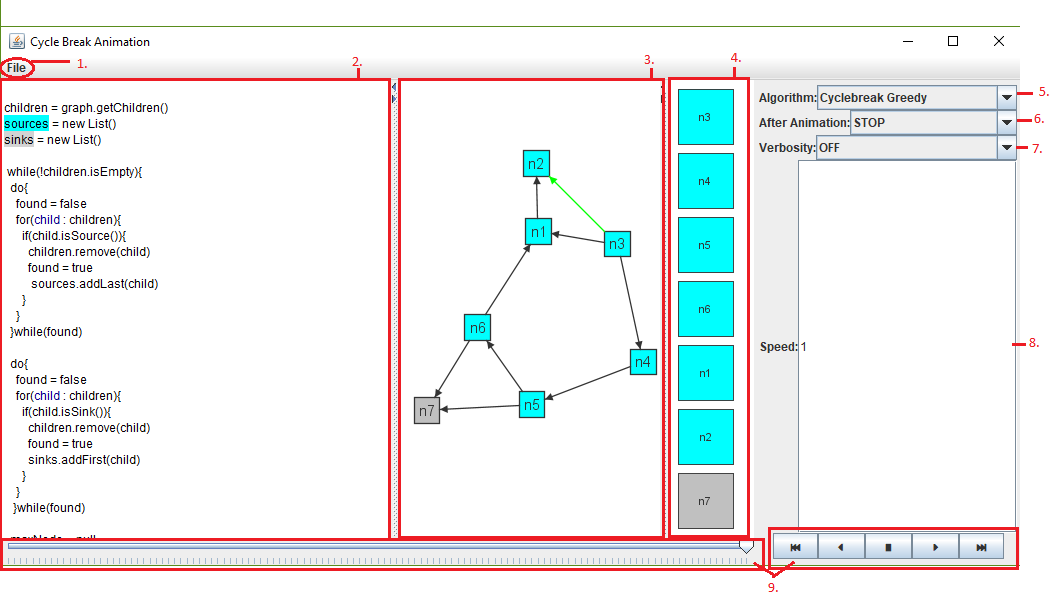
\includegraphics[width=\textwidth]{parts/InterfaceV2_1}

\begin{list}{-}{}
\item[1.] You can choos a file from the filesystem to be diplayed and you can save an animation for a loaded graph as a gif here
\item[2.] The current choosen algorithm is displayed here in pseudocode
\item[3.] A visual representation of the loaded full graph
\item[4.] A topological representation representation of the loaded graph
\item[5.] A list to choose a cycle break algorithm
\item[6.] Choose what should be done when autoplay reaches an end
\begin{list}{-}{}
\item[STOP] End the animation
\item[LOOP] Start the animation from the beginning
\item[REVERSE] Play the animation reversed
\end{list}
\item[7.] Choose verbosity of the steps of the animation
\begin{list}{-}{}
\item[OFF] Step funktion is disabled
\item[DEPTH 0-6] Steps stop when they reach the indent of the pseudocode with a number lesser or equal than the number of DEPTH
\end{list}
\item[8.] Set the speed the animation is displayed with
\item[9.] Slider and controls for the animation
\begin{list}{-}{}
\item[SLIDER] Displayes the current progress of the animation can be moved to display specific times in the animation
%\item[ \stepbackwards ]  TODO Unicode
%\item[⏮]
\item[ $| \! \! \! \blacktriangleleft \! \blacktriangleleft$ ] Plays the animation backwards till the Pseudocode reaches an indent set by verbosity
\item[ $\blacktriangleleft$ ] Plays the animation backwards till the end
\item[$ \blacksquare $] Stops the animation
\item[$ \blacktriangleright $] Plays the animation forwards
\item[$ \blacktriangleright \! \blacktriangleright \! \! \!|$]  Plays the animation forwards till the Pseudocode reaches an indent set by verbosity
\end{list}
\end{list}

%order of chapters not yet final
% where to put which file and what to do and not to do
\section{Guidlines}

These are our development guidlines.

\href{https://www.ietf.org/rfc/rfc2119.txt}{RFC2119}

\begin{list}{-}{}
\item The Project will be split into modules,

all modules MUST begin with \basemodule,

all packages in a modul MUST start with the modules name.

\item All main functions not for testing MUST be in the \basemodule[.main] module.

\item All test MUST be in the \basemodule[.test] module.

\item No module SHALL depend on the module \basemodule[.test]

\item No module SHALL but \basemodule[.test] MAY depend on the module \basemodule[.main]

\item Loading Graphs from file SHOULD be done in the \basemodule[.file] module

\item The Project SHOULD be implemented using the MVC pattern.

\item Models SHOULD be in the package \basemodule[.modle].

\item Views SHOULD be in the package \basemodule[.view].

\item Controllers SHOULD be in the package \basemodule[.control].

\item The module \basemodule[.api] SHOULD contain all api related stuff. %TODO

\item Code Comments and this Specification SHALL be in English.

\item The Algorithm MUST default to be deterministic.

\item Options that make the Algorithm none deterministic MUST be advanced/hidden.

\item For Randomness a PRNG SHALL be used with a configurable or fixed seed,
on re-runs the seed MUST be restored to it's initial value.

\item Magic constants SHOULD be avoided, instead use a commented constant.
\end{list}

% why are we doing what we are doing
\include{parts/Reasoning}

\section{Modules}

\begin{list}{-}{The Project consists of the following Modules}
\item \basemodule[.api]
\item \basemodule[.main]
\item \basemodule[.view]
\item \basemodule[.file.json]
\item \basemodule[.file.toml]
\item \basemodule[.algorithm.greedy]
\item \basemodule[.test]
\item \basemodule[.test.algorithm.force]
\end{list}

Required Direct Dependencies

\begin{adjustbox}{max width=\textwidth}
\begin{tabular}{|c|m{43mm}|m{70mm}|}
\hline 
\rule[-1ex]{0pt}{2.5ex} Module & External& Internal \\ 
\hline 
\rule[-1ex]{0pt}{2.5ex} \basemodule[.api] & org.eclipse.elk.graph \, org.eclipse.elk.alg.force & - \\ 
\hline 
\rule[-1ex]{0pt}{2.5ex} \basemodule[.main] & org.eclipse.elk.graph & \basemodule[.api] \, \basemodule[.view] \\ 
\hline 
\rule[-1ex]{0pt}{2.5ex} \basemodule[.view] & org.eclipse.elk.graph & \basemodule[.api] \\ 
\hline 
\rule[-1ex]{0pt}{2.5ex} \basemodule[.file.json] & org.eclipse.elk.graph.json & \basemodule[.api] \\ 
\hline 
\rule[-1ex]{0pt}{2.5ex} \basemodule[.file.toml] & org.eclipse.elk.graph \, toml4j & \basemodule[.api] \\ 
\hline 
\rule[-1ex]{0pt}{2.5ex} \basemodule[.algorithm.greedy] & org.eclipse.elk.graph \, org.eclipse.elk.core & \basemodule[.api] \, \basemodule[.view] \\ 
\hline 
\rule[-1ex]{0pt}{2.5ex} \basemodule[.test] & junit \, org.eclipse.elk.alg.force & \basemodule[.api] \, \basemodule[.main] \, \basemodule[.view] \, \basemodule[.file.json] \, \basemodule[.file.toml] \, \basemodule[.algorithm.greedy] \\ 
\hline 
\rule[-1ex]{0pt}{2.5ex} \basemodule[.test.algorithm.force] & org.eclipse.elk.graph \, org.eclipse.elk.core & \basemodule[.api] \, \basemodule[.view] \\ 
\hline 
\end{tabular}
\end{adjustbox}

\par

\basemodule[.main] also has optional runtime dependencies of two types, per type at least one should be present for our program to be useful.

The first Type is IAlgoritm which is implemented by \basemodule[.algorithm.greedy] or \basemodule[.test.algorithm.force].

The second Type is IGraphLoader wich is implemented by  \basemodule[.file.json] or \basemodule[.file.toml].


\section{File Formats}

We provide two implementations of the IGraphLoader service
which handles loading an ElkGraph from a File.

\subsection{\basemodule[.file.json]}

This module provides the IGraphLoader service for Json Files using the ElkJson Format which is documented \underline{\href{https://www.eclipse.org/elk/documentation/tooldevelopers/graphdatastructure/jsonformat.html}{here}}.

\subsection{\basemodule[.file.toml]}

This module provides the IGraphLoader service for v0.4.0 \underline{\href{https://github.com/toml-lang/toml}{Toml}} Files.

The root Toml Object/Table represents the root node which
has the same requirements as any other node.

\paragraph{Node Fields}
\begin{tabular}{|c|c|c|}
\hline 
Field Name & Type & Default/Required \\ 
\hline 
id & String & Required \\ 
\hline 
no\_layout & boolean & Default false \\ 
\hline 
x & double & Default 0.0 \\ 
\hline 
y & double & Default 0.0 \\ 
\hline 
width & double & Default 0.0 \\ 
\hline 
height & double & Default 0.0 \\ 
\hline 
children & Array of Tables(Nodes) & Default Empty Array \\ 
\hline 
edges & Array of Tables(Edges) & Default Empty Array \\ 
\hline 
\end{tabular} 

\paragraph{Edge Fields}
\begin{tabular}{|c|c|c|}
\hline 
Field Name & Type & Default/Required \\ 
\hline 
id & String & Required \\ 
\hline 
targets & Array of Strings & Required Not Empty \\ 
\hline 
sources & Array of Strings & Required Not Empty \\ 
\hline 
\end{tabular} 

The Strings in an Edges targets and sources field are the ids of Nodes.

\paragraph{}
All fields not listed here are ignored.
% How we use the the Graph and how we perform cycle breaking
\section{Model}
The Model contains the following properties:
\begin{list}{-}{}
\item Performs choosen cycle break algorithm in another thread
\item Can return graph with Property that edges were reversed
\item The state of the Graph per "Step" will be saved

\end{list}



% How we represent the the Graph and animate the steps
\section{View}
The UI will be looking like: \\
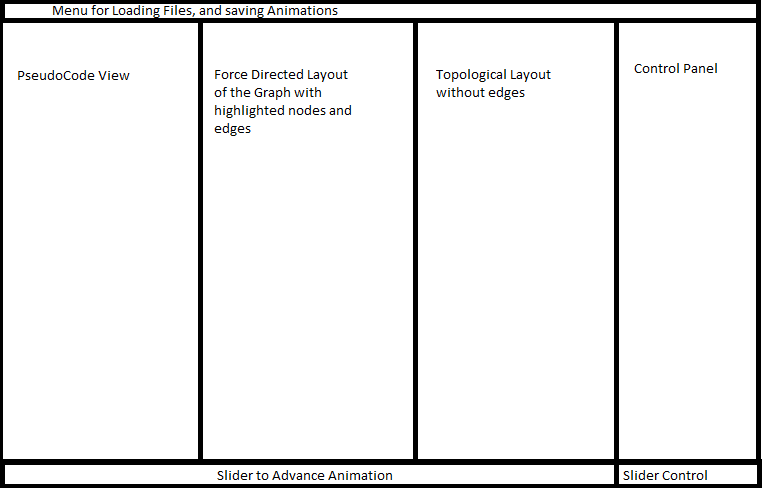
\includegraphics[width=\textwidth]{parts/UIFinished}
\begin{list}{-}{}
\item The left section will be showing the pseudocode of the current active algorithm.
\item The middle sections will show one force directed  graph on the left that will higlight Nodes the right will be ordered Topological.

\item Nodes in both graphs will be coloured dynamically.
\begin{list}{-}{}
\item Currently used node will be coloured blue in the left graph.
\item Sources will be colured cyan.
\item Sinks will be colured light gray.
\end{list}
\item Edges will be coloured as following.
\begin{list}{-}{}
\item Active edge will be coloured blue.
\item Reversed edges will be coloured green.
\end{list}
\item The right section will be a Control Panel.
\begin{list}{-}{}
\item for more information see Section Controller

\end{list}
\end{list}





% How we influence the representation
\section{Controller}
The Control panel contains:
\begin{list}{-}{}
\item A dropdown list with cycle-break algorithms
\item An option to choose verbosity
\item A slider to jump to a part of the animation
\item An option to choose how fast autoplay is
\item Buttons to play the animation forward, backward and stopping the animation
\item Buttons to step backward and and forward

\end{list}


\section{Model}
The Model contains the following properties:
\begin{list}{-}{}
\item The state of the Graph per "Step" will be saved

\end{list}






\section{Classes}



% This needs to be done
\section{Minimal Viable Product}

\begin{list}{-}{}
\item A Cycle Break algorithm (Greedy)
\item Load a graph from a file (In your own input format)
\item Present a drawing of the graph
\item Be able to configure the verbosity of the animation (step forwards or backwards, run continuously, speed, level of detail, ...)
\item Be well-structured, i.e. in terms of separation of concerns (drawing, layout calculation, ...)
\item implement your visualization application in Java Swing

\item use the ElkGraph as the input format for your visualization.


\item comment the code
\end{list} % Minimum Viable Product
\end{document}